Smita Darmora defended her Ph.D. thesis on the search for stop in August, 2015. Her work was supervised by PI De and base funded researcher Guilio Usai. The title of her thesis was: ``SEARCH FOR A SUPERSYMMETRIC PARTNER TO THE TOP QUARK
USING A MULTIVARIATE ANALYSIS TECHNIQUE.'' 

Figure~\ref{smita_limit} shows the 95\% confidence limit exclusion limit for a 300 GEV mass stop.

\begin{figure}[hbt]
  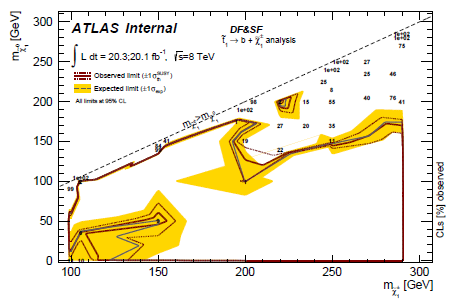
\includegraphics[width=\linewidth]{smita_limit.png}
  \caption{Exclusion limit for a 300 GeV mass stop obtained by combining MET trigger and Lepton trigger samples from a Ph.D.  thesis written by Smita Darmora.}
  \label{smita_limit}
\end{figure}
